% Transmisión de video desde el módulo de captura al dispositivo del alumno.
% Se compila por separado: pdflatex transmision_video.tex -> transmision_video.pdf
\documentclass[tikz,border=6pt]{standalone}
\usepackage[utf8]{inputenc}
\usepackage[T1]{fontenc}
\usepackage{cmbright}
\usepackage{graphicx}
\usetikzlibrary{arrows.meta,calc,fit,backgrounds}

\definecolor{azul}{RGB}{20,50,120}
\definecolor{tarjeta}{RGB}{236,238,252}
\definecolor{borde}{RGB}{200,205,235}
\definecolor{cvideo}{RGB}{130,50,140}
\definecolor{cpedido}{RGB}{25,80,190}

\begin{document}
\begin{tikzpicture}[
    font=\normalsize,
    caja/.style={draw=borde, line width=0.8pt, fill=tarjeta, rounded corners=5pt,
                 inner sep=5pt, align=center, text=azul, minimum width=3.4cm},
    msg/.style={font=\small, align=center},
    >={Stealth[length=7pt]}
]

% ---------------- Módulo de captura ----------------
\node (cam) at (0,0) {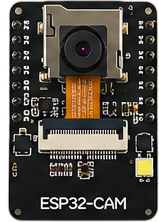
\includegraphics[height=2.6cm]{red_esp32cam.png}};

% Captura continua
\node[caja] (sensor) at (3.6,1.45)  {\textbf{Cámara}\\{\small fotograma de 320x240 píxeles}};
\node[caja] (jpeg)   at (3.6,0)     {\textbf{Codificador JPEG}\\{\small por hardware}};
\node[caja] (buf)    at (3.6,-1.45) {\textbf{Búfer en PSRAM}\\{\small último fotograma}};
\draw[->, azul, line width=1.2pt] (sensor) -- (jpeg);
\draw[->, azul, line width=1.2pt] (jpeg) -- (buf);

% Envío, solo mientras hay una petición
\node[caja, minimum width=2.8cm] (srv) at (7.6,-1.45) {\textbf{Servidor HTTP}\\{\small puerto 80}};
\node[caja, minimum width=2.8cm] (led) at (7.6,0.75)  {\textbf{LED IR}};
\draw[->, azul, line width=1.2pt] (buf) -- node[msg, above, text=azul] {toma} (srv);
\draw[->, azul, line width=1.2pt] (srv) -- node[msg, right, text=azul] {enciende\\y apaga} (led);

\begin{scope}[on background layer]
  \node[draw=azul, line width=1pt, dashed, rounded corners=8pt, inner sep=9pt,
        fit=(cam)(sensor)(jpeg)(buf)(srv)(led)] (mc) {};
\end{scope}
\node[text=azul, font=\large\bfseries, anchor=south] at (mc.north) {Módulo de captura};
\node[text=azul, font=\small, anchor=north] at (mc.south) {192.168.4.50};

% ---------------- Dispositivo del alumno ----------------
\coordinate (alu) at (16.4,-1.45);
\begin{scope}[shift={(alu)}, azul, line width=1.5pt]
  \draw[rounded corners=3pt] (-0.45,-0.85) rectangle (0.45,0.85);
  \fill (0,-0.68) circle (0.06);
\end{scope}
\node[text=azul, align=center, anchor=south] at ($(alu)+(0,1.0)$) {\textbf{Dispositivo}\\\textbf{del alumno}};

% ---------------- Pedido ----------------
\draw[->, cpedido, line width=1.3pt] ($(alu)+(-0.65,0.5)$) -- node[msg, above, text=cpedido]
     {Petición HTTP\\\texttt{GET /stream}} ($(mc.east |- alu)+(0,0.5)$);

% ---------------- Flujo de fotogramas ----------------
\draw[->, cvideo, line width=1.3pt] ($(mc.east |- alu)+(0,-0.5)$) -- ($(alu)+(-0.65,-0.5)$);
\foreach \i in {0,1,2} {
  \begin{scope}[shift={($(mc.east |- alu)+(0.6+1.45*\i,-0.5)$)}]
    \draw[cvideo, fill=white, line width=0.8pt] (0,-0.3) rectangle (1.1,0.3);
    \fill[cvideo!25] (0.01,0.29) rectangle (0.24,-0.29);
    \node[font=\scriptsize, text=cvideo] at (0.67,0) {JPEG};
  \end{scope}
}
\node[msg, text=cvideo, anchor=north] at ($(mc.east |- alu)+(2.8,-0.95)$) {Flujo continuo de fotogramas (MJPEG)};

\end{tikzpicture}
\end{document}
